\chapter{الحركية الكيميائية: قوانين السرعة}\label{ch:b1:rate-laws}

يحتفظ الحليب بجودته أسبوعًا في الثلاجة ويومًا على مائدة صيفية. وتقول علبة
الدواء «يُحفظ دون \qty{25}{\celsius}» وتحمل تاريخ
صلاحية بعد سنتين أو ثلاث، لم يكن للصانع وقت
لرصده مباشرة. فثوابت التوازن تقول أين ينتهي التفاعل؛
ولا تقول شيئًا عن المدة التي يستغرقها لبلوغ ذلك. وهذا ميدان
الحركية الكيميائية. يعرّف هذا الفصل \omterm{def:b1:rate-laws:rate}{سرعة التفاعل}، \omterm{def:b1:rate-laws:order}{وقوانين
السرعة} التي تعبّر عنها بدلالة التراكيز، والصيغ المكاملة
التي تتنبأ بالتراكيز في كل لحظة، والطرائق التجريبية التي
تحدد \omterm{def:b1:rate-laws:order}{قانون السرعة}، \omterm{thm:b1:rate-laws:arrhenius}{وقانون أرهينيوس} الذي يصف أثر
درجة الحرارة --- وهو الأداة التي يُتنبأ بها بمدة صلاحية الدواء
في بضعة أسابيع من التجارب.

\begin{recall}
قدّم الكتاب الأول (الصف الثاني عشر) سرعة ظهور نوع
وسرعة اختفائه، والعوامل الحركية (التركيز، ودرجة الحرارة، والحفاز)
\omterm{def:b1:rate-laws:half-life}{وزمن نصف التفاعل} لتفاعل من الرتبة الأولى. وقد عُرّف \omterm{def:b1:extent-q-and-k:extent}{تقدم التفاعل} $\xi$
في \cref{def:b1:extent-q-and-k:extent}.
\end{recall}

\begin{omfigure}
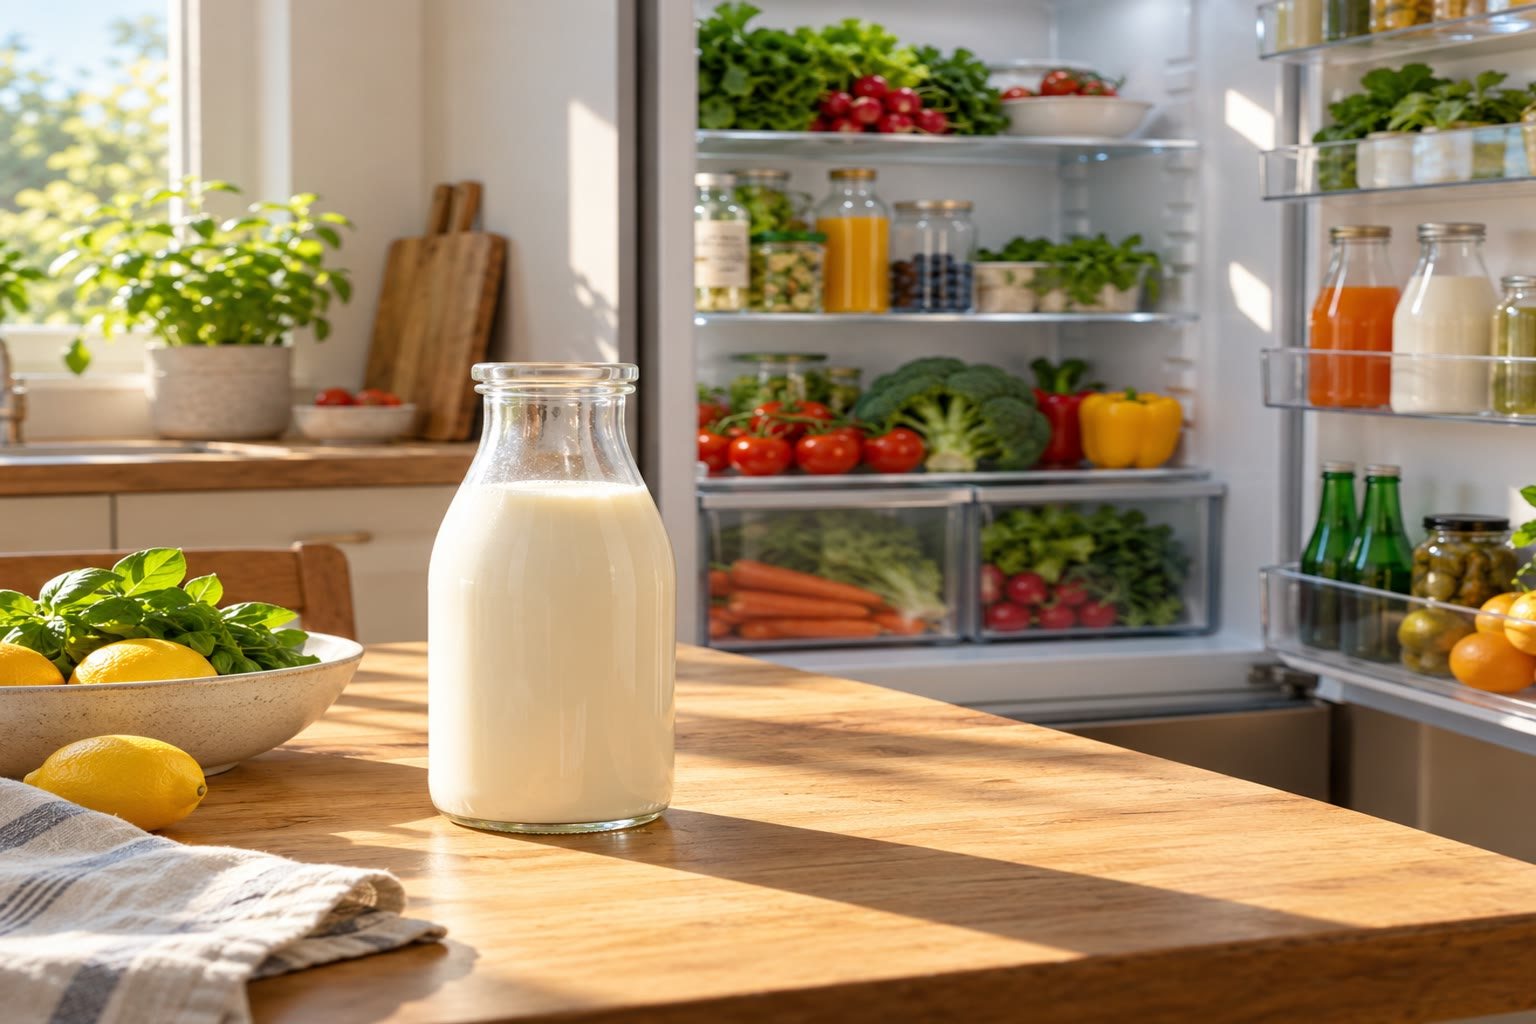
\includegraphics[width=0.55\linewidth]{images/book2/ai/b1-08-milk-kitchen.jpg}

{\small قارورة حليب متروكة في الشمس بجوار ثلاجة مفتوحة.
فالتفاعلات التي تفسده تجري في حرارة الصيف أسرع بعدة
مرات منها في البرد.}
\end{omfigure}

\section{سرعة التفاعل}

\begin{definition}[سرعة التفاعل، سرعتا التكوّن والاختفاء]\label{def:b1:rate-laws:rate}
من أجل تفاعل $0 = \sum_i \nu_i\mathrm{A}_i$ يجري في مفاعل
مغلق حجمه ثابت $V$، تكون \emph{سرعة التفاعل}\index{سرعة التفاعل}
هي
\[
  v = \frac{1}{V}\frac{\dd\xi}{\dd t} = \frac{1}{\nu_i}\frac{\dd[\mathrm{A}_i]}{\dd t}
  \quad\text{أيًّا كان } i\text{},
\]
بالوحدة \unit{mol.L^{-1}.s^{-1}}. و\emph{سرعة تكوّن}\index{سرعة التكوّن}
ناتج هي $\dd[\mathrm{A}_i]/\dd t$؛ و\emph{سرعة
اختفاء}\index{سرعة الاختفاء} متفاعل هي
$-\dd[\mathrm{A}_i]/\dd t$.
\end{definition}

\begin{proposition}[سرعة واحدة لكل الأنواع]\label{prop:b1:rate-laws:rate-relations}
لا تتعلق \omterm{def:b1:rate-laws:rate}{سرعة التفاعل} بالنوع المختار لتتبعه:
فمن أجل $a\,\mathrm{A} + b\,\mathrm{B} \longrightarrow c\,\mathrm{C} + d\,\mathrm{D}$،
\[
  v = -\frac1a\frac{\dd[\ce{A}]}{\dd t} = -\frac1b\frac{\dd[\ce{B}]}{\dd t}
  = \frac1c\frac{\dd[\ce{C}]}{\dd t} = \frac1d\frac{\dd[\ce{D}]}{\dd t} .
\]
\end{proposition}

\begin{proof}
$[\mathrm{A}_i] = (n_{i,0} + \nu_i\xi)/V$ مع $V$ ثابت، فيكون
$\dd[\mathrm{A}_i]/\dd t = (\nu_i/V)\,\dd\xi/\dd t = \nu_i v$.
\end{proof}

\begin{example}[تفكك خماسي أكسيد ثنائي النيتروجين]\label{ex:b1:rate-laws:n2o5}
من أجل \ce{2N2O5 -> 4NO2 + O2}: $v = -\frac12\frac{\dd[\ce{N2O5}]}{\dd t} =
\frac14\frac{\dd[\ce{NO2}]}{\dd t} = \frac{\dd[\ce{O2}]}{\dd t}$. فيظهر ثنائي أكسيد
النيتروجين بسرعة تعادل أربعة أضعاف سرعة ظهور ثنائي الأكسجين، ويختفي خماسي أكسيد ثنائي النيتروجين
بسرعة تعادل ضعف سرعة ظهور ثنائي الأكسجين.
\end{example}

\section{قوانين السرعة والرتب}

\begin{definition}[قانون السرعة، الرتب، ثابت السرعة]\label{def:b1:rate-laws:order}
\emph{قانون السرعة}\index{قانون السرعة} يعبّر عن السرعة دالةً في
التراكيز. ويقال إن للتفاعل \emph{رتبة} حين يأخذ قانون سرعته
الشكل
\[
  v = k\,[\mathrm{A}]^{p}\,[\mathrm{B}]^{q} \cdots ;
\]
تكون الأسس $p$، $q$، \dots\ \emph{الرتب الجزئية}\index{رتبة جزئية}
بالنسبة إلى A وB و\dots، ومجموعها \emph{الرتبة
الكلية}\index{رتبة كلية}، و$k$ هو \emph{ثابت السرعة}\index{ثابت السرعة}،
الذي لا يتعلق إلا بدرجة الحرارة. وتُعيَّن الرتب
تجريبيًا؛ ولا يلزم أن تساوي المعاملات الستوكيومترية، وقد
تكون كسرية أو معدومة.
\end{definition}

\begin{remark}[وحدات $k$]\label{rem:b1:rate-laws:units}
بما أن $v$ بالوحدة \unit{mol.L^{-1}.s^{-1}}، فإن $k$ بالوحدة
\unit{mol.L^{-1}.s^{-1}} للرتبة 0، و\unit{s^{-1}} للرتبة 1،
و\unit{L.mol^{-1}.s^{-1}} للرتبة 2، وعمومًا
$(\unit{mol/L})^{1-n}\,\unit{s^{-1}}$ \omterm{def:b1:rate-laws:order}{للرتبة الكلية} $n$. فوحدة
$k$ تدل على \omterm{def:b1:rate-laws:order}{الرتبة الكلية}.
\end{remark}

\begin{remark}[تفاعلات بلا رتبة]\label{rem:b1:rate-laws:no-order}
ليس لكل تفاعل رتبة. فسرعة بعض التفاعلات كسر
في مقامه تراكيز، أو تتعلق بتركيز
ناتج. وتفسَّر \omterm{def:b1:rate-laws:order}{قوانين السرعة} هذه
بآلية التفاعل (\cref{ch:b1:elementary-steps}). وقد يكون
للتفاعل رتبة في بدايته فقط: هي \omterm{def:b1:rate-laws:order}{قانون السرعة} الابتدائي.
\end{remark}

\section{قوانين السرعة المكاملة وأزمنة نصف التفاعل}

\begin{definition}[زمن نصف التفاعل]\label{def:b1:rate-laws:half-life}
\emph{زمن نصف التفاعل}\index{زمن نصف التفاعل} $t_{1/2}$ لمتفاعل هو المدة
التي يكون قد استُهلك بعدها نصف كميته الابتدائية.
\end{definition}

\begin{theorem}[قوانين السرعة المكاملة]\label{thm:b1:rate-laws:integrated}
من أجل تفاعل $a\mathrm{A} \rightarrow \text{نواتج}$ سرعته $v = -\frac1a\frac{\dd[\ce{A}]}
{\dd t} = k[\ce{A}]^n$، مع $[\ce{A}](0) = a_0$:
\begin{center}
\begin{tabular}{llll}
\hline
الرتبة & القانون المكامل & التمثيل الخطي & \omterm{def:b1:rate-laws:half-life}{زمن نصف التفاعل} \\
\hline
0 & $[\ce{A}] = a_0 - akt$ & $[\ce{A}]$ بدلالة $t$ & $a_0/(2ak)$ \\
1 & $[\ce{A}] = a_0\,\eu^{-akt}$ & $\ln[\ce{A}]$ بدلالة $t$ & $\ln2/(ak)$ \\
2 & $\dfrac{1}{[\ce{A}]} = \dfrac{1}{a_0} + akt$ & $1/[\ce{A}]$ بدلالة $t$ & $1/(ak\,a_0)$ \\
\hline
\end{tabular}
\end{center}
\end{theorem}

\begin{proof}
لنكتب $c = [\ce{A}]$، فيكون $\dd c/\dd t = -akc^n$.
\emph{الرتبة 0}: $\dd c/\dd t = -ak$، ومنه $c = a_0 - akt$ (صالحة حتى
$c = 0$). \emph{الرتبة 1}: $\dd c/\dd t = -akc$ معادلة تفاضلية خطية
من الرتبة الأولى حلها $c = a_0\eu^{-akt}$.
\emph{الرتبة 2}: $\dd c/c^2 = -ak\,\dd t$؛ وبالمكاملة من 0 إلى $t$،
$-1/c + 1/a_0 = -akt$، فيكون $1/c = 1/a_0 + akt$. أزمنة نصف التفاعل: نضع $c =
a_0/2$ في كل قانون ونحلّ بالنسبة إلى $t$.
\end{proof}

\begin{proposition}[اختبار زمن نصف التفاعل]\label{prop:b1:rate-laws:half-life-test}
لا يتعلق \omterm{def:b1:rate-laws:half-life}{زمن نصف التفاعل} بالتركيز الابتدائي إلا إذا كان
التفاعل من الرتبة 1، وعندئذ فقط. وهو متناسب مع $a_0$ في الرتبة 0
ومع $1/a_0$ في الرتبة 2. والتفاعل من الرتبة الأولى يفقد نصف ما تبقى
في كل \omterm{def:b1:rate-laws:half-life}{زمن نصف تفاعل} متتالٍ: فبعد $m$ زمنًا من أزمنة نصف التفاعل يبقى الكسر $2^{-m}$.
\end{proposition}

\begin{proof}
من أجل الرتبة $n \ne 1$، يعطي فصل المتغيرات $t_{1/2} = \dfrac{2^{n-1} -
1}{(n-1)\,ak\,a_0^{n-1}}$، الذي يتعلق بالتركيز $a_0$ ما لم يكن $n = 1$؛ ومن أجل
$n = 1$، $t_{1/2} = \ln2/(ak)$. وفي الرتبة 1، $c(t + t_{1/2}) = c(t)/2$ عند
كل $t$، لأن $\eu^{-ak(t + t_{1/2})} = \eu^{-akt}/2$.
\end{proof}

\begin{omfigure}
\begin{tikzpicture}
\begin{axis}[name=p0,
  width=0.36\linewidth, height=4.6cm,
  xmin=0, xmax=60, ymin=0, ymax=1.05,
  axis x line=bottom, axis y line=left,
  xlabel={\babelsublr{$t$ (min)}}, title={\foreignlanguage{arabic}{الرتبة \babelsublr{0}: $[\ce{A}]$}},
  title style={font=\small}, xtick={0,20,40,60},
  tick label style={font=\scriptsize}, label style={font=\small}]
\addplot[omDef, thick] table[x=t, y=A0] {figdata/out/bachelor-1-integrated-rate-laws.dat};
\end{axis}
\begin{axis}[at={(p0.east)}, anchor=west, xshift=0.9cm, name=p1,
  width=0.36\linewidth, height=4.6cm,
  xmin=0, xmax=60, ymin=-3.2, ymax=0.2,
  axis x line=bottom, axis y line=left,
  xlabel={\babelsublr{$t$ (min)}}, title={\foreignlanguage{arabic}{الرتبة \babelsublr{1}: $\ln[\ce{A}]$}},
  title style={font=\small}, xtick={0,20,40,60},
  tick label style={font=\scriptsize}, label style={font=\small}]
\addplot[omProp, thick] table[x=t, y=lnA1] {figdata/out/bachelor-1-integrated-rate-laws.dat};
\end{axis}
\begin{axis}[at={(p1.east)}, anchor=west, xshift=0.9cm,
  width=0.36\linewidth, height=4.6cm,
  xmin=0, xmax=60, ymin=0, ymax=4.2,
  axis x line=bottom, axis y line=left,
  xlabel={\babelsublr{$t$ (min)}}, title={\foreignlanguage{arabic}{الرتبة \babelsublr{2}: $1/[\ce{A}]$}},
  title style={font=\small}, xtick={0,20,40,60},
  tick label style={font=\scriptsize}, label style={font=\small}]
\addplot[omThm, thick] table[x=t, y=invA2] {figdata/out/bachelor-1-integrated-rate-laws.dat};
\end{axis}
\end{tikzpicture}

\begin{tikzpicture}
\begin{axis}[
  width=0.62\linewidth, height=5.0cm,
  xmin=0, xmax=60, ymin=0, ymax=1.05,
  axis x line=bottom, axis y line=left,
  xlabel={\babelsublr{$t$ (min)}}, ylabel={\babelsublr{$[\ce{A}]$ (mol/L)}}, xtick={0,10,20,30,40,50,60},
  tick label style={font=\small}, label style={font=\small},
  legend style={font=\small, draw=none, at={(0.98,0.98)}, anchor=north east}]
\addplot[omDef, thick] table[x=t, y=A0] {figdata/out/bachelor-1-integrated-rate-laws.dat};
\addplot[omProp, thick] table[x=t, y=A1] {figdata/out/bachelor-1-integrated-rate-laws.dat};
\addplot[omThm, thick] table[x=t, y=A2] {figdata/out/bachelor-1-integrated-rate-laws.dat};
\legend{{\foreignlanguage{arabic}{الرتبة \babelsublr{0}}}, {\foreignlanguage{arabic}{الرتبة \babelsublr{1}}}, {\foreignlanguage{arabic}{الرتبة \babelsublr{2}}}}
\draw[dotted] (axis cs:0,0.5) -- (axis cs:20,0.5);
\end{axis}
\end{tikzpicture}

{\small ثلاثة تفاعلات لها التركيز الابتدائي نفسه
(\qty{1.00}{mol/L}) \omterm{def:b1:rate-laws:initial-rate}{والسرعة الابتدائية} نفسها
(\qty{0.050}{mol.L^{-1}.min^{-1}}). في الأعلى: يصير كل قانون مكامل
مستقيمًا في إحداثياته الخاصة. في الأسفل: التراكيز؛ وأزمنة
نصف التفاعل 10 و13.9 و20 دقيقة.}
\end{omfigure}

\section{تعيين قانون السرعة}

\begin{method}[الطريقة التكاملية]\label{met:b1:rate-laws:integral}
لاختبار رتبة بقياسات $[\ce{A}](t)$: ارسم $[\ce{A}]$
و$\ln[\ce{A}]$ و$1/[\ce{A}]$ بدلالة $t$؛ فالتمثيل الذي يكون
مستقيمًا يعطي الرتبة، وميله يعطي $k$ (الميل $-ak$ أو $-ak$ أو $+ak$
على الترتيب).
\end{method}

\begin{method}[طريقة زمن نصف التفاعل]\label{met:b1:rate-laws:half-life}
قِس \omterm{def:b1:rate-laws:half-life}{زمن نصف التفاعل} من أجل عدة تراكيز ابتدائية: إن كان ثابتًا
فالرتبة 1؛ وإن كان متناسبًا مع $a_0$ فالرتبة 0؛ وإن كان متناسبًا مع $1/a_0$ فالرتبة
2. وفي تجربة واحدة، قارن المدة اللازمة للانتقال من $a_0$ إلى $a_0/2$
بالمدة اللازمة للانتقال من $a_0/2$ إلى $a_0/4$: فتساويهما يعني الرتبة 1.
\end{method}

\begin{definition}[السرعة الابتدائية]\label{def:b1:rate-laws:initial-rate}
\emph{السرعة الابتدائية}\index{سرعة ابتدائية} $v_0$ هي السرعة عند $t = 0$،
وتُقرأ ميلًا للمماس عند المبدأ للمنحنى $[\ce{A}](t)$،
مقسومًا على المعامل الستوكيومتري. وفي تلك اللحظة تكون
التراكيز هي التراكيز الابتدائية المعلومة ولا يتدخل أي ناتج.
\end{definition}

\begin{method}[طريقة السرعات الابتدائية]\label{met:b1:rate-laws:initial-rates}
من أجل $v_0 = k[\ce{A}]_0^p[\ce{B}]_0^q$: أجرِ تجارب لا يتغير فيها
إلا $[\ce{A}]_0$؛ فيكون $\ln v_0 = \ln(k[\ce{B}]_0^q) + p\ln[\ce{A}]_0$،
وميل $\ln v_0$ بدلالة $\ln[\ce{A}]_0$ هو $p$. وعمليًا،
مضاعفة $[\ce{A}]_0$ تضرب $v_0$ في $2^p$. وافعل الشيء نفسه مع B.
\end{method}

\begin{definition}[طريقة العزل، الرتبة الظاهرية]\label{def:b1:rate-laws:apparent-order}
في \emph{طريقة العزل}\index{طريقة العزل} توضع المتفاعلات كلها إلا
واحدًا بإفراط كبير (عشرة أضعاف أو أكثر). فتبقى تراكيزها
ثابتة عمليًا، ويكون $v = k[\ce{A}]^p[\ce{B}]^q \approx k'[\ce{A}]^p$
مع $k' = k[\ce{B}]_0^q$: فيسلك التفاعل سلوك تفاعل
\emph{رتبته الظاهرية}\index{رتبة ظاهرية} $p$ وثابت سرعته الظاهري
$k'$. ويسمى ذلك أيضًا انحطاط الرتبة.
\end{definition}

\begin{omfigure}
\begin{tikzpicture}
\begin{axis}[
  width=0.55\linewidth, height=4.8cm,
  xmin=0, xmax=40, ymin=0, ymax=1.05,
  axis x line=bottom, axis y line=left,
  xlabel={\babelsublr{$t$ (min)}}, ylabel={\babelsublr{$[\ce{A}]$ (mol/L)}},
  xtick={0,10,20,30,40},
  tick label style={font=\small}, label style={font=\small}, clip mode=individual]
\addplot[omProp, thick] table[x=t, y=A1] {figdata/out/bachelor-1-integrated-rate-laws.dat};
\draw[omThm, thick] (axis cs:0,1) -- (axis cs:20,0);
\node[omThm, anchor=west, font=\small] at (axis cs:2,0.12) {\foreignlanguage{arabic}{المماس عند $t = 0$}};
\end{axis}
\end{tikzpicture}

{\small قراءة \omterm{def:b1:rate-laws:initial-rate}{سرعة ابتدائية}: يلتقي المماس عند المبدأ (بالأحمر) لمنحنى
من الرتبة الأولى بمحور الزمن عند $t_0 = \qty{20}{min}$، فيكون $v_0 =
\qty{1.00}{mol/L}/\qty{20}{min} = \qty{0.050}{mol.L^{-1}.min^{-1}}$.}
\end{omfigure}

\begin{inthelab}[تتبّع تفاعل مع الزمن]
يُبنى \omterm{def:b1:rate-laws:order}{قانون السرعة} من تراكيز تقاس أثناء جريان التفاعل.
فحين يكون متفاعل أو ناتج ملوّنًا، يسجّل مطياف ضوئي
الامتصاصية، المتناسبة مع تركيزه (بير--لامبرت،
\cref{ch:b1:structure-spectroscopy})؛ وحين تظهر أيونات أو تختفي،
يتتبع مقياس الموصلية الموصلية؛ وحين يتكوّن غاز في وعاء
مغلق، يتتبع مقياس الضغط الضغط. وإلا تؤخذ عيّنات في
أزمنة معلومة، ويوقَف التفاعل (يُخمَد) بالتبريد أو بالتخفيف،
وتُعاير كل عيّنة. وتُبقى درجة حرارة الوعاء
ثابتة بحمام منظَّم الحرارة، لأن $k$ يتعلق بها تعلقًا شديدًا.
\end{inthelab}

\section{درجة الحرارة: قانون أرهينيوس}

\begin{definition}[طاقة التنشيط]\label{def:b1:rate-laws:activation-energy}
تُعرَّف \emph{طاقة التنشيط}\index{طاقة التنشيط} $E_a$ لتفاعل
ثابت سرعته $k(T)$ بالعلاقة
\[
  \frac{\dd \ln k}{\dd T} = \frac{E_a}{RT^2} ,
\]
بالوحدة \unit{J/mol}. وحين لا تتعلق $E_a$ بدرجة الحرارة $T$، تعطي المكاملة
$k = A\,\eu^{-E_a/RT}$، حيث الثابت $A$، الذي له وحدة $k$، هو
\emph{العامل قبل الأسي}\index{عامل قبل أسي}.
\end{definition}

\begin{theorem}[قانون أرهينيوس]\label{thm:b1:rate-laws:arrhenius}
في أغلب التفاعلات، وعلى مجال معتدل من درجات الحرارة، يتبع \omterm{def:b1:rate-laws:order}{ثابت
السرعة} \emph{قانون أرهينيوس}\index{قانون أرهينيوس}
\[
  k(T) = A\,\eu^{-E_a/RT} ,
\]
مع $A$ و$E_a > 0$ مستقلين عن $T$: فيكون $\ln k$ دالة خطية في
$1/T$ ميلها $-E_a/R$.
\end{theorem}
\admitted

\begin{remark}[معنى $E_a$]\label{rem:b1:rate-laws:meaning}
القانون تجريبي. وتفسيره --- أن الاصطدامات الجزيئية التي
تحمل طاقة من رتبة $E_a$ على الأقل هي وحدها التي تؤدي إلى التفاعل، وأن
كسر هذه الاصطدامات يتغير كما $\eu^{-E_a/RT}$ --- يُرسم إجمالًا
مع مخططات الطاقة في الفصل التالي، ثم تجعله \omterm{def:b1:extent-q-and-k:quantitative}{كمّيًا}
نظريات سرعات التفاعل في مجلد السنة الثالثة.
\end{remark}

\begin{method}[تعيين $E_a$]\label{met:b1:rate-laws:arrhenius-plot}
انطلاقًا من \omterm{def:b1:rate-laws:order}{ثوابت سرعة} عند عدة درجات حرارة، ارسم $\ln k$ بدلالة $1/T$
(بالكلفن): فالميل هو $-E_a/R$، والجزء المقطوع $\ln A$. ومع درجتي
حرارة فقط،
\[
  E_a = \frac{R\,\ln(k_2/k_1)}{1/T_1 - 1/T_2} .
\]
\end{method}

\begin{example}[قاعدة تقريبية]\label{ex:b1:rate-laws:doubling}
من أجل $E_a = \qty{53}{kJ/mol}$، يضرب الانتقال من 25 إلى \qty{35}{\celsius}
الثابتَ $k$ في $\exp\!\big(\frac{53000}{8.314}(\frac{1}{298.15} -
\frac{1}{308.15})\big) = 2.0$. فالقاعدة المألوفة «عشر درجات زيادة، سرعة
مضاعفة» تصح قرب درجة حرارة الغرفة في التفاعلات التي طاقة تنشيطها
نحو \qty{50}{kJ/mol}؛ وإذا كانت $E_a$ أكبر كان العامل أكبر.
\end{example}

\begin{omfigure}
\begin{tikzpicture}
\begin{axis}[
  width=0.6\linewidth, height=5.4cm,
  xmin=2.95, xmax=3.45, ymin=-9.0, ymax=-4.2, clip mode=individual,
  axis x line=bottom, axis y line=left,
  xlabel={\babelsublr{$1000/T$ (\unit{K^{-1}})}}, ylabel={\foreignlanguage{arabic}{$\ln k$، و$k$ بالوحدة \unit{d^{-1}}}},
  xtick={3.0,3.1,3.2,3.3,3.4}, ytick={-9,-8,-7,-6,-5},
  tick label style={font=\small}, label style={font=\small}]
\addplot[omDef, thick] table[x=invT_1e3, y=lnk] {figdata/out/bachelor-1-arrhenius-line.dat};
\addplot[only marks, mark=*, mark size=2.2pt, omThm] table[x=invT_1e3, y=lnk] {figdata/out/bachelor-1-arrhenius-points.dat};
\node[font=\small, anchor=south west] at (axis cs:3.002,-4.71) {\qty{60}{\celsius}};
\node[font=\small, anchor=south west] at (axis cs:3.095,-5.66) {\qty{50}{\celsius}};
\node[font=\small, anchor=south west] at (axis cs:3.193,-6.67) {\qty{40}{\celsius}};
\draw[dashed, black!50] (axis cs:3.354,-9.0) -- (axis cs:3.354,-8.31);
\addplot[only marks, mark=o, mark size=2.4pt, omDef] coordinates {(3.354,-8.310)};
\node[font=\small, anchor=east] at (axis cs:3.33,-8.40) {\foreignlanguage{arabic}{\qty{25}{\celsius}، بالاستكمال}};
\end{axis}
\end{tikzpicture}

{\small تمثيل أرهينيوس لتفكك دواء (مسألة نهاية
الأسبوع): تقع ثلاثة \omterm{def:b1:rate-laws:order}{ثوابت سرعة} مقيسة (بالأحمر) على مستقيم ميله
$-E_a/R$؛ وبمدّه إلى \qty{25}{\celsius} يعطي مدة الصلاحية في
درجة حرارة الغرفة.}
\end{omfigure}

\begin{history}[أرهينيوس، 1889]
اقترح الكيميائي السويدي سفانته أرهينيوس، وهو يدرس قلب السكروز بالأحماض
سنة 1889، أن كسرًا صغيرًا فقط من الجزيئات، هي التي
في حالة «منشَّطة»، يتفاعل، وأن هذا الكسر يكبر مع
درجة الحرارة كما $\eu^{-E/RT}$. وصارت الفكرة، المثيرة للجدل أول الأمر،
أساس الحركية الكيميائية. ونال أرهينيوس جائزة نوبل في
الكيمياء سنة 1903 عن نظريته في التفكك الإلكتروليتي.
\end{history}

\begin{omfigure}
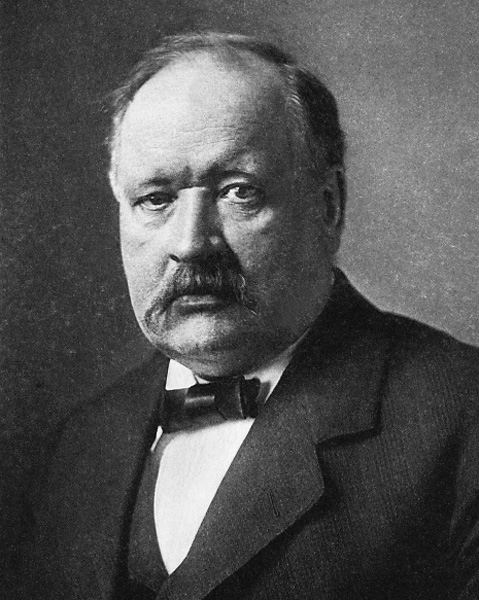
\includegraphics[width=0.22\linewidth]{images/book2/arrhenius.jpg}

{\small سفانته أرهينيوس (1859--1927)، سنة 1909.}
\end{omfigure}

\section{تمارين}

\begin{exercise}[$\star$]\label{exo:b1:rate-laws:1}
من أجل \ce{2N2O5 -> 4NO2 + O2} بحجم ثابت، يظهر ثنائي أكسيد النيتروجين بالسرعة
$\qty{2.0e-4}{mol.L^{-1}.s^{-1}}$. أعطِ \omterm{def:b1:rate-laws:rate}{سرعة التفاعل}، \omterm{def:b1:rate-laws:rate}{وسرعة
تكوّن} ثنائي الأكسجين، \omterm{def:b1:rate-laws:rate}{وسرعة اختفاء} \ce{N2O5}.
\end{exercise}

\begin{exercise}[$\star$]\label{exo:b1:rate-laws:2}
أعطِ وحدة \omterm{def:b1:rate-laws:order}{ثابت السرعة} من أجل الرتب الكلية 0 و1 و2 و3،
والتراكيز بالوحدة \unit{mol/L} والأزمنة بالثواني.
\end{exercise}

\begin{exercise}[$\star$]\label{exo:b1:rate-laws:3}
لتفاعل من الرتبة الأولى $\mathrm{A} \longrightarrow \mathrm{B}$ الثابت $k = \qty{3.0e-3}{s^{-1}}$. احسب
زمن نصف تفاعله والكسر المتبقي من \ce{A} بعد \qty{10}{min}.
\end{exercise}

\begin{exercise}[$\star$]\label{exo:b1:rate-laws:4}
حين يُنصَّف التركيز الابتدائي لمتفاعل، يتضاعف زمن نصف تفاعله. ما
الرتبة؟ وماذا لو انتصف \omterm{def:b1:rate-laws:half-life}{زمن نصف التفاعل}؟
\end{exercise}

\begin{exercise}[$\star\star$]\label{exo:b1:rate-laws:5}
يقاس تركيز متفاعل \ce{A} ($\mathrm{A} \longrightarrow \mathrm{P}$): عند $t
= 0$ و10 و20 و30 و\qty{40}{min}، $[\ce{A}] = 0.100$ و0.0741 و0.0549
و0.0407 و\qty{0.0301}{mol/L}. عيّن الرتبة \omterm{def:b1:rate-laws:order}{وثابت
السرعة}.
\end{exercise}

\begin{exercise}[$\star\star$]\label{exo:b1:rate-laws:6}
من أجل $\mathrm{A} + \mathrm{B} \longrightarrow \mathrm{P}$، $v_0 = \qty{2.0e-6}{mol.L^{-1}.s^{-1}}$ عندما $[\ce{A}]_0
= [\ce{B}]_0 = \qty{0.010}{mol/L}$؛ و\qty{8.0e-6}{} حين يُضاعَف $[\ce{A}]_0$؛
و\qty{4.0e-6}{} حين يُضاعَف $[\ce{B}]_0$. أوجد \omterm{def:b1:rate-laws:order}{الرتب
الجزئية} \omterm{def:b1:rate-laws:order}{وقانون السرعة} \omterm{def:b1:rate-laws:order}{وثابت السرعة}.
\end{exercise}

\begin{exercise}[$\star\star$]\label{exo:b1:rate-laws:7}
قانون \omterm{def:b1:rate-laws:rate}{سرعة التفاعل} $\mathrm{A} + \mathrm{B} \longrightarrow \mathrm{P}$ هو $v = k[\ce{A}][\ce{B}]$. ومع
$[\ce{B}]_0 = \qty{0.50}{mol/L}$ و$[\ce{A}]_0 = \qty{5.0e-3}{mol/L}$،
يختفي \ce{A} وفق حركية من الرتبة الأولى بثابت ظاهري
\qty{0.012}{s^{-1}}. فسّر واحسب $k$.
\end{exercise}

\begin{exercise}[$\star\star$]\label{exo:b1:rate-laws:8}
\omterm{def:b1:rate-laws:order}{ثابت سرعة} قيمته \qty{1.0e-3}{s^{-1}} عند \qty{300}{K}
و\qty{5.0e-3}{s^{-1}} عند \qty{320}{K}. احسب \omterm{def:b1:rate-laws:activation-energy}{طاقة التنشيط}
\omterm{def:b1:rate-laws:order}{وثابت السرعة} عند \qty{310}{K}.
\end{exercise}

\begin{exercise}[$\star\star$]\label{exo:b1:rate-laws:9}
للتفاعل $2\,\mathrm{A} \longrightarrow \mathrm{P}$ \omterm{def:b1:rate-laws:order}{قانون السرعة} $v = -\frac12\frac{\dd[\ce{A}]}
{\dd t} = k[\ce{A}]^2$ مع $k = \qty{0.50}{L.mol^{-1}.s^{-1}}$. انطلاقًا
من $[\ce{A}]_0 = \qty{0.020}{mol/L}$، احسب \omterm{def:b1:rate-laws:half-life}{زمن نصف التفاعل}
والتركيز بعد \qty{100}{s}.
\end{exercise}

\begin{exercise}[$\star\star\star$]\label{exo:b1:rate-laws:10}
بيّن أن المدة اللازمة لاستهلاك كسر $f$ من المتفاعل، في تفاعل من الرتبة الأولى،
هي $t_f = -\ln(1 - f)/(ak)$. وقارن
المدد اللازمة لاستهلاك 50\,\% و75\,\% و90\,\% و99.9\,\%، معبَّرًا عنها بأزمنة نصف التفاعل.
\end{exercise}

\begin{exercise}[$\star\star\star$]\label{exo:b1:rate-laws:11}
تحرر لصيقة جلدية دواءً بسرعة ثابتة
\qty{0.40}{mg/h} ما دام خزانها، الذي يحوي في البداية \qty{10}{mg}، غير
فارغ. اكتب قانون الكمية المتبقية، وأعطِ رتبته وزمن نصف تفاعله
والمدة التي تنفد بعدها اللصيقة. ولماذا تلائم الحركية من الرتبة صفر
لصيقة الدواء؟
\end{exercise}

\begin{exercise}[$\star\star\star$]\label{exo:b1:rate-laws:12}
بيّن أن القاعدة «عشر درجات زيادة، سرعة مضاعفة» بين
\qty{298.15}{K} و\qty{308.15}{K} توافق $E_a \approx
\qty{53}{kJ/mol}$. ما العامل الذي تعطيه \omterm{def:b1:rate-laws:activation-energy}{طاقة التنشيط} نفسها
بين \qty{0}{\celsius} و\qty{10}{\celsius}؟
\end{exercise}

\section{مسألة: مدة صلاحية دواء}

\begin{problem}[{مسألة نهاية الأسبوع --- اختبار ثباتية معجَّل:
تفكك من الرتبة الأولى عند 60\,\textdegree C، وثلاث درجات حرارة،
وتمثيل أرهينيوس، ومدة الصلاحية في درجة حرارة الغرفة}]
\label{pb:b1:rate-laws:1}
للتنبؤ بمدة الصلاحية $t_{90}$ لقرص دوائي (المدة التي يكون قد تفكك بعدها 10\,\%
من المادة الفعالة)، يحفظ مختبر عيّنات عند
درجة حرارة عالية ويقيس النسبة المئوية المتبقية من المادة الفعالة. عند
\qty{60}{\celsius}:
\begin{center}
\begin{tabular}{lccccc}
\hline
الزمن (يوم) & 0 & 10 & 20 & 30 & 40 \\
المادة الفعالة المتبقية (\%) & 100.0 & 91.4 & 83.5 & 76.3 & 69.8 \\
\hline
\end{tabular}
\end{center}
وعند 40 و\qty{50}{\celsius} تكون \omterm{def:b1:rate-laws:order}{ثوابت السرعة} المعيَّنة
\qty{1.27e-3}{d^{-1}} و\qty{3.48e-3}{d^{-1}}. خذ $R =
\qty{8.314}{J/(mol.K)}$ والشهر $= \qty{30.4}{d}$.

\medskip
\noindent\textbf{الجزء الأول --- الرتبة عند 60\,\textdegree C.}
\begin{enumerate}
  \item احسب الخسائر على كل فترة من 10 أيام. هل التفاعل من
        الرتبة 0؟
  \item احسب $\ln(\%\text{ المتبقية})$ عند كل زمن. ماذا تستنتج؟
  \item استنتج \omterm{def:b1:rate-laws:order}{ثابت السرعة} $k_{60}$.
  \item احسب \omterm{def:b1:rate-laws:half-life}{زمن نصف التفاعل} عند \qty{60}{\celsius}.
  \item ما النسبة المئوية المتبقية بعد 60 يومًا عند \qty{60}{\celsius}؟
  \item احسب $t_{90}$ عند \qty{60}{\celsius}.
\end{enumerate}

\medskip
\noindent\textbf{الجزء الثاني --- مدة الصلاحية والرتبة.}
\begin{enumerate}[resume]
  \item بيّن أن $t_{90} = \ln(10/9)/k$ في تفكك من الرتبة الأولى.
  \item عبّر عن $t_{90}$ كسرًا من \omterm{def:b1:rate-laws:half-life}{زمن نصف التفاعل}.
  \item لماذا لا تتعلق $t_{90}$ بجرعة القرص؟
  \item لماذا تقيس المختبرات التفكك عند درجة حرارة عالية
        لا عند \qty{25}{\celsius}؟
  \item لو كان التفكك من الرتبة 2 بالنسبة إلى المادة الفعالة، فهل يدوم
        قرص مضاعف القوة أطول أم أقل؟ فسّر.
\end{enumerate}

\medskip
\noindent\textbf{الجزء الثالث --- تمثيل أرهينيوس.}
\begin{enumerate}[resume]
  \item اجعل في جدول قيم $1/T$ و$\ln k$ للدرجات الثلاث.
  \item احسب ميل المستقيم المار بنقطتي 40
        و\qty{60}{\celsius}.
  \item استنتج \omterm{def:b1:rate-laws:activation-energy}{طاقة التنشيط}.
  \item تحقق من أن نقطة \qty{50}{\celsius} تقع على المستقيم.
  \item احسب \omterm{def:b1:rate-laws:activation-energy}{العامل قبل الأسي} $A$.
  \item بأي عامل تزداد السرعة بين 25
        و\qty{35}{\celsius}؟ قارن بالقاعدة التقريبية.
\end{enumerate}

\medskip
\noindent\textbf{الجزء الرابع --- درجة حرارة الغرفة.}
\begin{enumerate}[resume]
  \item مدّد \omterm{def:b1:rate-laws:order}{ثابت السرعة} إلى \qty{30}{\celsius}.
  \item احسب $t_{90}$ عند \qty{30}{\celsius}، بالأشهر.
  \item نُسيت علبة ثلاثة أيام في سيارة عند \qty{60}{\celsius}. ما
        الكسر المفقود من المادة الفعالة؟
  \item فسّر التعليمة «يُحفظ دون \qty{25}{\celsius}».
  \item مدّد \omterm{def:b1:rate-laws:order}{ثابت السرعة} إلى \qty{25}{\celsius}.
  \item احسب مدة الصلاحية $t_{90}$ عند \qty{25}{\celsius}، بالأيام
        وبالأشهر.
\end{enumerate}
\end{problem}
